\documentclass[10pt,twocolumn,letterpaper]{article}

%%%%%%%%% PAPER TYPE  - PLEASE UPDATE FOR FINAL VERSION
% \usepackage[review]{cvpr}      % To produce the REVIEW version
% \usepackage{cvpr}              % To produce the CAMERA-READY version
\usepackage[pagenumbers]{cvpr} % To force page numbers, e.g. for an arXiv version

% Include other packages here, before hyperref.
\usepackage{graphicx}
\usepackage{amsmath}
\usepackage{amssymb}
\usepackage{booktabs}
\usepackage{tablefootnote}
\usepackage{booktabs}
\graphicspath{{"../results/"}}

% It is strongly recommended to use hyperref, especially for the review version.
% hyperref with option pagebackref eases the reviewers' job.
% Please disable hyperref *only* if you encounter grave issues, e.g. with the
% file validation for the camera-ready version.
%
% If you comment hyperref and then uncomment it, you should delete
% ReviewTempalte.aux before re-running LaTeX.
% (Or just hit 'q' on the first LaTeX run, let it finish, and you
%  should be clear).
\usepackage[pagebackref,breaklinks,colorlinks]{hyperref}
\DeclareMathSizes{10}{8.5}{4}{2}


% Support for easy cross-referencing
\usepackage[capitalize]{cleveref}
\crefname{section}{Sec.}{Secs.}
\Crefname{section}{Section}{Sections}
\Crefname{table}{Table}{Tables}
\crefname{table}{Tab.}{Tabs.}


%%%%%%%%% PAPER ID 
\def\cvprPaperID{*****} % *** Enter the CVPR Paper ID here
\def\confName{CVPR}
\def\confYear{2022}


\begin{document}

%%%%%%%%% TITLE
\title{Robust transmission expansion assessment using minimal samples}

\author{Erich Trieschman\\
Stanford University, Department of Statistics\\
{\tt\small etriesch@stanford.edu}
% \and
% Second Author\\
% Institution2\\
% First line of institution2 address\\
% {\tt\small secondauthor@i2.org}
}
\maketitle

%%%%%%%%% ABSTRACT
\begin{abstract}
\end{abstract}
  

%------------------------------------------------------------------------
\section{Introduction}
\label{sec:intro}

In re-structured electricity markets in the United States, transmission system planning is conducted through the joint collaboration between regulatory agencies and an Independent System Operator (ISO)\cite{grid_lab_transmission_2023}. Through Integrated Resource Planning (IRP) proceedings, Load Serving Entities (LSE's) and regulatory agencies use capacity expansion models to optimize sequential investment decisions in thermal, renewable, and storage plant capacity over decades into the future\cite{hobbs_adaptive_2016}. Capacity expansion and production cost planning models require forecasts of load, resource availability, and costs to serve as constraints to be met through the dispatch of resources over a transmission network. However, current planning methods often rely on a single or few scenarios of load and resource availability forecasts. While deterministic models can help communicate a single system cost estimates, their results are highly sensitive to model inputs and ignore uncertainty in future conditions. 

To address this challenge, methods in decision-making under uncertainty have been developed for electricity transmission system planning. The Transmission Economic Assessment Methodology (TEAM)\cite{zhang_using_2010} framework offers a solution to address uncertainties in transmission planning. One pillar of TEAM seeks to manage uncertainty by stress-testing transmission alternatives across potential future scenarios in a stochastic production cost simulation with high nodal resolution. The explicit uncertainty analysis proposed in TEAM includes fuel costs, renewable resource availability, thermal unit availability, and future load to produce an output distribution of system costs for which risk metrics can be derived. However, these approaches are computationally expensive given the calculation of the operational expenses under many stochastic variables and the high-resolution network model needed to characterize transmission economic benefits adequately.

In this project, we focus on methods to select a subset of optimal load, wind, and solar forecasts to characterize the cost-benefit distribution of a transmission expansion project. Given a distribution of correlated load, wind, and solar scenarios, we use experimental design and active learning techniques to minimize the subset of forecasts required to characterize the distribution of system costs of an expansion decision. Our primary objective is to evaluate these methods under a single transmission expansion scenario, which we will optimize under the expected value of the forecasts. 

We use a 97-bus synthetic network of the Western Electricity Coordinating Council (WECC) to assess the benefits of developing a High Voltage Direct Current transmission line to integrate floating offshore wind from California's north coast.

We are able to approximate the cost-benefit distributions after only 25-50 samples. Assuming that an adequate distribution can be generated with 500 samples, this represents computational savings of 90-95\%. We also find that the optimal methods we explore approximate these cost-benefit distributions significantly better than baselines of randomly selected sample points.

%------------------------------------------------------------------------
\section{Methods}
\label{sec:methods}
This work aims to efficiently generate distributions of economic benefits from transmission expansion scenarios using a nodal production cost simulation (PCS). To achieve this, we use techniques from experiment design and active learning to fit surrogate models to the production cost simulation outputs.

To generate our target empirical distribution of benefits (hereafter "true distribution"), we first determine the optimal transmission expansion under the expected value of the solar, wind, and load profiles. We then run a large sample of model inputs through the cost model. This is the computationally expensive step, which we wish to improve upon. 

To generate our estimated empirical distribution of benefits (hereafter "surrogate distribution"), we fit surrogate models to a subset of cost model runs and run a large sample of model inputs through the surrogate model, which we expect to realize significant computational gains. See Figure \ref{fig:methods} for an overview of our approaches, which we describe in the subsections below

\begin{figure}[!htbp]
    \centering
    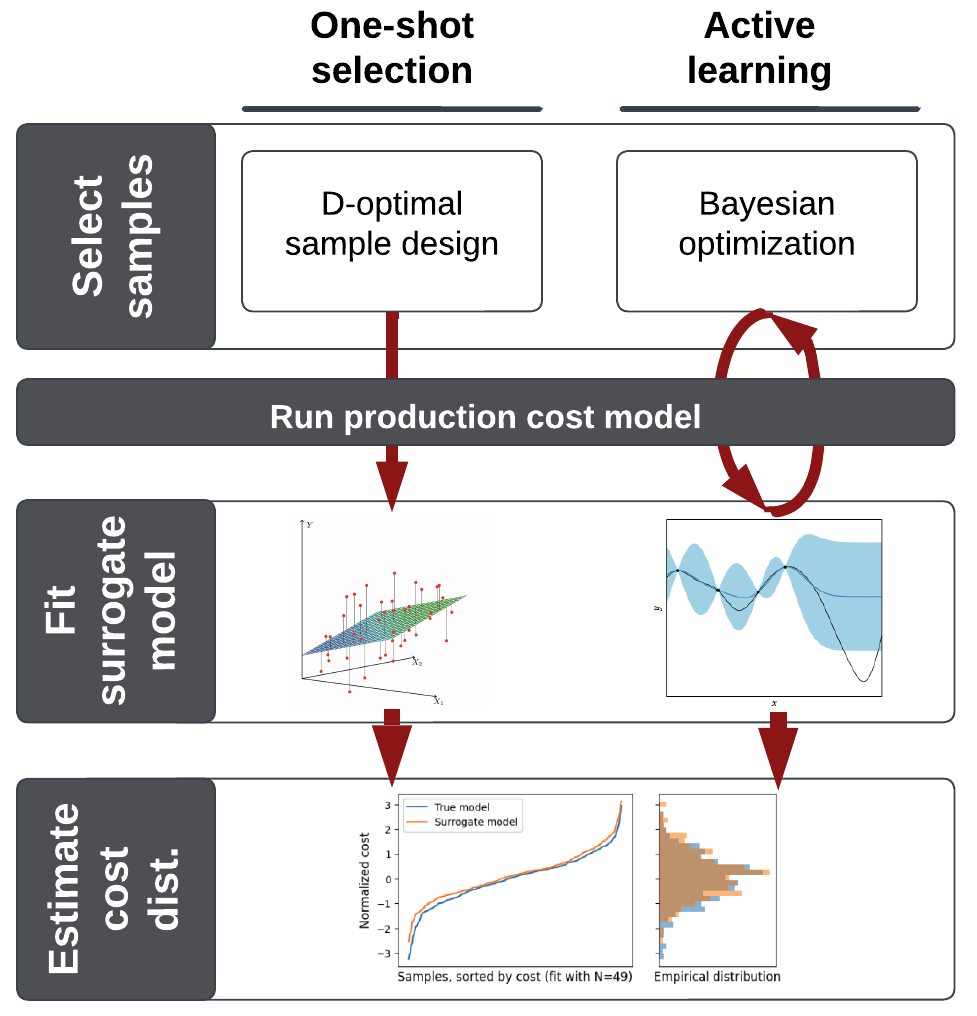
\includegraphics[scale=0.2]{methods_diagram.png}
    \caption{\label{fig:methods}Methods used to estimate empirical distributions}
\end{figure}

\subsection{Production cost simulation and model inputs}

The PCS is built on the pypsa-usa Breakthrough Energy synthetic Western Electricity Coordinating Council (WECC) network model\cite{xu_us_2020}. The PCS is an operational simulation of the electricity transmission system that provides information on the techno-economic performance of a power system, such as system operating costs, market prices, transmission congestion, and more. Figure \ref{fig:network} shows the network we model.

\begin{align*}
    \text{Benefits} &=  \tilde{\lambda}_{n,t} \cdot P_{\text{load}} - \lambda_{n,t} \cdot P_{\text{load}} \\
    &\underbrace{\phantom{\text{Benefits}}}_{\text{HVDC Expansion}} \hspace{1em} \underbrace{\phantom{\text{Benefits}}}_{\text{Pre-expansion}}
 \end{align*}
    

\begin{figure}[h]
    \centering
    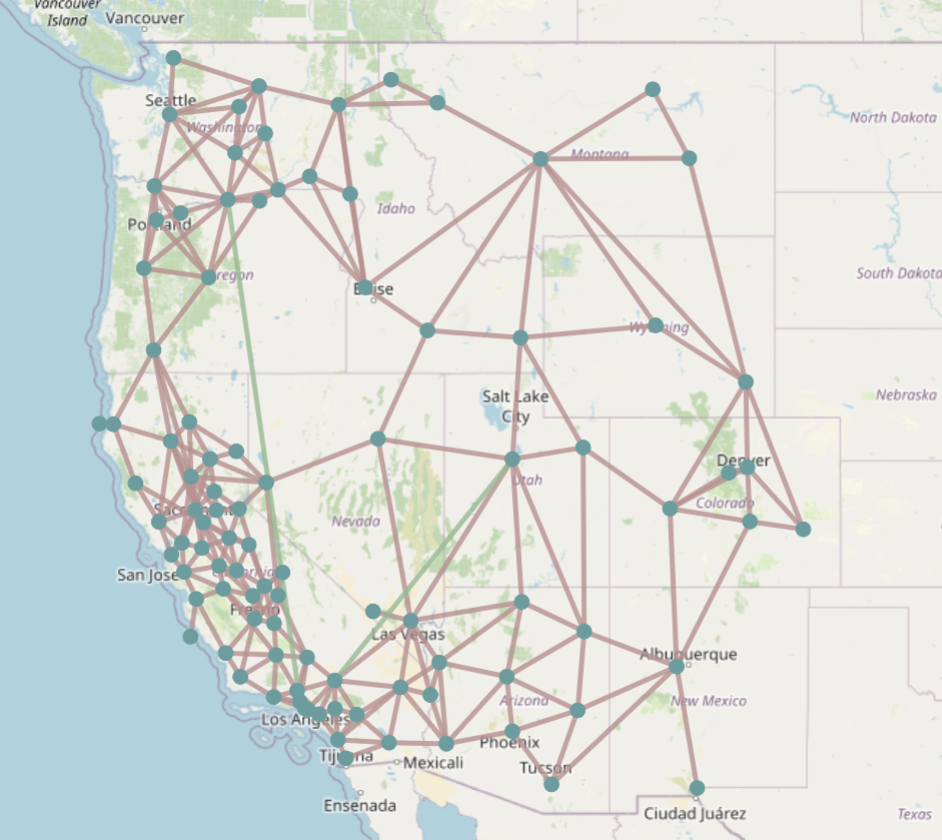
\includegraphics[scale=0.25]{network.png}
    \caption{pypsa-usa 96-node WECC network}
    \label{fig:network}
\end{figure}

We generate stochastic load, wind, and solar profiles using the mean-reversion stochastic process method developed by the CAISO\cite{liu_order_nodate,liu_stochastic_2016}. This method uses a stochastic process-based method to generate profiles representing deviations from an expected base profile. We use the data embedded in the Breakthrough Energy network from 2016 as the "base" hourly load, wind, and solar profiles.

Estimating system costs for just a small subset of nodes over a single year results in a massive number of model inputs (8760 hours in a year $\times$ 3 time series $\times$ 20 nodes $>$ 500,000 inputs). To overcome the curse of dimensionality, we use Principal Component Analysis (PCA) to encode the input data and drastically reduce the sample space. Our goal is to reduce the number of dimensions to a target of 10 dimensions, while retaining the important features of the original data. 

PCA is a widely used data reduction technique that identifies linear combinations of input features that capture the most significant variation in the data. This method begins with an eigendecomposition of the covariance matrix of the dataset. The eigenvectors represent the directions along which the data varies the most, while the eigenvalues represent the amount of variation along each of these directions. The eigenvectors with the largest eigenvalues capture the most variation in the data, and are referred to as the principal components once they are normalized. Encoding with PCA involves projecting the original data onto a subset these principal components, which reduces the dimensionality of the dataset while preserving as much of the original variation as possible.

Encoded data, $Y \in \mathbb{R}^{n\times D}$, can be formed as 
\begin{align*}
    X^TX &= Q\Lambda Q^{-1} \textrm{, the covariance eigendecomposition}\\
    U &\in \mathbb{R}^{n\times n}, \textrm{ s.t. } u_i = \frac{q_i}{\lVert q_i \rVert} \textrm{ for } Q = [q_1, \dots, q_n]\\
    Y &= XU_D \textrm{, for } U_D = [u_1, \dots, u_D]
\end{align*}

Operation of the production cost simuation (hearafter "cost model") and generation of the encoded stochastic load, wind, and solar profiles (hereafter "model inputs") is conducted outside the scope of this project. 

\subsection{Scenario selection}
To evaluate the performance of our scenario selection methods, we compare their surrogate distributions to the true distribution. We also compare each to a baseline, which is trained with a random sample of model inputs; we expect the baseline surrogate distributions to differ more from the true distribution.

We propose two optimal scenario selection methods. These methods are used to generate surrogate models, which approximate the computationally expensive cost model. Surrogate distributions can then be generated by the entire sample of forecasts through the inexpensive surrogate models. The first optimal scenario selection approach is taken from the literature of experiment design. We refer to this approach as "One-shot selection" as it selects all samples at the outset of the surrogate model training. The second optimal scenario selection approach is taken from the literature of active learning and we refer to it as such. Active learning selection sequentially selects optimal forecasts based on uncertainty in the surrogate model output being fit.

\subsubsection{One-shot selection}
In this approach we assume a linear relationship between forecasts and transmission cost outputs and use the surrogate cost model 
\begin{align*}
    y_i = x_i^T\beta + \epsilon_i, \text{ with } y_i \in \mathbb{R}, \; x_i, \beta \in \mathbb{R}^n, \; \epsilon \text{ white noise }
\end{align*} 

We estimate $\hat{\beta}$ using maximum likelihood estimation and minimize the uncertainty of our estimator $\hat{\beta}$ by minimizing the inverse covariance of our input data. Assuming a fixed set of $p$ input data combinations, $v_j$, and $M$ desired scenarios to be selected, we may select target input data to minimize the inverse covariance by optimizing the following problem:
\begin{align*}
\min_m. \; (\textrm{over } S_+) \quad & \left(\sum_{j=1}^pm_jv_jv_j^T\right)^{-1}\\
s.t. \quad & m \succeq 0, \; m^T1 = M, \; m \in \{0, 1\}^n
\end{align*}

Here, $m\in \mathbb{R}^p$ is an indicator variable whos $j^{th}$ entry determines whether scenarios $v_j$ is selected. We choose $m \in \{0, 1\}^n$ instead of the canonical formulation, $m \in \mathbb{Z}^n$, because our cost model is deterministic and we only need to concern ourselves with a single selection for each scenario.

We scalarize the problem with the D-optimal design formulation as described in Boyd et. al. \cite{boyd}. We also relax the binary constraint using the L1-norm heuristic, replacing $m$ with $\lambda$ in our formulation to represent this. We choose the L1-norm constraint instead of the cannonical constraint $\lambda^T1 = \alpha M$ to maximize sparsity in the resulting solution, since we seek a solution with up to one choice per input scenario. 
\begin{align*}
    \min_\lambda. \quad & -\log\det \left(\sum_{j=1}^p\lambda_jv_jv_j^T\right)\\
    s.t. \quad & 0 \preceq \lambda \preceq 1, \quad \lVert\lambda\rVert _1 \leq \alpha M
\end{align*}

This relaxed problem may yield a solution $\lambda_i \in [0, 1]$. We choose the input data scenarios with the $M$ largest values in $\lambda$ to run through the cost model.

There are two design choices for this problem, which we care to explore in future work. First, we must choose how to discretize continuous input data, $x_i$, into finite input data scenarios, $v_j$. We choose 10 data bins for each dimension and a uniform split across bins. Second, we must choose hyperparameter $\alpha$ to control the impact of the L1-heuristic constraint; we use $\alpha=2$. 

\subsubsection{Active learning selection}
Active learning design is a sequential approach to selecting optimal scenarios for the cost model. In this approach, we iteratively select forecasts to run through the cost model based on the previous forecasts and the cost model outputs.

One popular method for active learning selection is Bayesian optimization, which we use here. This approach estimates a probability distribution over cost function outputs, conditional on all of the previous model outputs; it does so through a Gaussian Process (GP) model, which is updated after each evaluation of the function. The selection of the next forecast is determined by an "acquisition function", defined by the objective we seek to optimize \cite{brochu2010tutorial} \cite{wang2022intuitive}. 

We define the Gaussian Process surrogate model as
\begin{align*}
    f(x) \sim \mathcal{GP}(0, k(x, x'))
\end{align*}

Where $x$ are the model inputs, and $k(x, x')$ is a pre-defined covariance function, often the squared exponential function, $k(x^{(i)}, x^{(j)}) = \exp\left(-\frac{1}{2}\lVert x^{(i)} - x^{(j)}\rVert^2_2\right)$. Assuming 0-mean is common in Bayesian optimization.

A property of the Gaussian Process is that any finite collection of model outputs follows a multivariate Normal distribution. Namely
\begin{align*}
    \begin{bmatrix}
        f(x^{(1)})\\\vdots\\f(x^{(n)})
    \end{bmatrix} := \textbf{f}^{(1:n)} \sim N(0, \textbf{K})
\end{align*}
Where $\textbf{K}\in \mathbb{R}^{n\times n}$ is the covariance matrix of the model inputs with $\textbf{K}_{ij} = k(x^{(i)}, x^{(j)})$.

Using the Sherman-Morrison-Woodbury formula and properties of conditional multivariate Normal distributions, we may generate the predictive probability of our surrogate cost model, given a model input and the evidence:
\begin{align*}
    f^{(n+1)} \mid \textbf{x}^{(1:n+1)} &\sim \mathcal{N}(\mu_{n+1}, v_{n+1}) \textrm{, where}\\
    \mu_{n+1} &:= \textbf{k}(x^{(n+1)})^T\textbf{K}^{-1}\textbf{f}^{(1:n)}\\
    v_{n+1} &:= k(x^{(n+1)}, x^{(n+1)}) - \textbf{k}(x^{(n+1)})^T\textbf{K}^{-1}\textbf{k}(x^{(n+1)})\\
    \textbf{k}(x^{(n+1)}) &:= \left[k(x^{(n+1)}, x^{(1)}), \dots, k(x^{(n+1)}, x^{(n)})\right]
\end{align*}

In our setting, we use Maximum Entropy Search (MES) as the acquisition function, which allows us to identify the forecast connected to the point of highest entropy in the surrogate cost model. Entropy is a measure of uncertainty about a given model input, so sequentially selecting maximal entropy points allows us to reduce overall uncertainty across our surrogate model \cite{sebastiani_mes}\cite{mussmann2018relationship}. We first derive an analytical form of the entropy equation, $H(f | \textbf{x}^{1:n}, x)$:
\begin{align*}
    H(f \mid \textbf{x}^{(1:n)}, x) :=& -\int N(f \mid \mu_x, v_x) \log\left[N(f \mid \mu_x, v_x)\right]df\\
    =& -\int N(f \mid \mu_x, v_x) \left[-\frac{1}{2}\log(2\pi v_x) - \frac{(f - \mu_x)^2}{2v_x}\right]df\\
    =& \frac{1}{2}\log(2\pi v_x) + \frac{1}{2}
\end{align*}

Using kernel $k(x^{(i)}, x^{(j)}) = \exp\left(-\frac{1}{2l^2}\lVert x^{(i)} - x^{(j)}\rVert^2_2\right)$, the point of maximum entropy in the surrogate model, $x^*$, is therefore
\begin{align*}
    &\; \textrm{argmax}_x \;\; \frac{1}{2}\log(2\pi v_x) + \frac{1}{2} = \; \textrm{argmax}_x \;\; v_x \\
    =&\; \textrm{argmax}_x \;\; k(x, x) - \textbf{k}(x)^T\textbf{K}^{-1}\textbf{k}(x)\\
    =&\; \textrm{argmin}_x \;\; \sum_{i=1}^n\sum_{j=1}^n \textbf{K}^{-1}_{ij} \textbf{k}(x)_i \textbf{k}(x)_j\\
    =&\; \textrm{argmin}_x \;\; \sum_{i=1}^n\sum_{j=1}^n C_{ij} \exp\left(-\frac{1}{l^2}\lVert x - \frac{1}{2}(x_i + x_j)\rVert _2^2\right)\\
    &\textrm{where } C_{ij} = \textbf{K}^{-1}_{ij}\exp(-\frac{1}{4l^2}\lVert x_i - x_j\rVert^2_2)
\end{align*}

This problem is clearly not convex, however, we employ several search strategies to approximate $x^*$ with $\hat{x}^*$. First we consider a brute force approach where we calculate entropy for a fixed set of sample points, $x \in \mathcal{D}$. $\hat{x}^*$ is simply the sample point yielding the maximal entropy. We also consider sequential convex programming (SCP) techniques using second order Taylor approximations and particle methods; these local methods leverage convex optimization theory.

In SCP we form a convex relaxation to the objective function, $f(x) = \sum_{ij} C_{ij} \exp\left(-\lVert x - \frac{1}{2}(x_i + x_j)\rVert _2^2\right)$, at each step of the optimization, and we iterate until local convergence. The update step in this optimization routine becomes
\begin{align*}
    x^{(n+1)^{(k+1)}} &= \textrm{argmin}_x \hat{f}^{(k)}(x) \;\; \textrm{s.t} \;\; x \in \mathcal{T}^{(k)}
\end{align*}
Where $\mathcal{T}^{(k)} := \{x \mid \lvert x_i - x_i^{(n+1)^{(k)}}\rvert \leq \rho^{(k)}_i\}$ is the convex trust region for the problem. Hyperparameter, $\rho^{(k)}$ is updated through the cannonical trust region update:
\begin{align*}
    \rho^{(k+1)} &= 
    \begin{cases}
        \beta^{succ}\rho^{(k)} & \text{if } \delta \geq \alpha \hat{\delta}\\
        \beta^{fail}\rho^{(k)} & \text{else}
    \end{cases} \text{, for }\\
    \delta &:= f\left(x^{(n+1)^{(k)}}\right) - f\left(x^{(n+1)^{(k+1)}}\right)\\
    \hat{\delta} &:= f\left(x^{(n+1)^{(k)}}\right) - \hat{f}^{(k)}\left(x^{(n+1)^{(k+1)}}\right)
\end{align*}

Practitioners often set $x^{(n+1)^{(k+1)}} \leftarrow x^{(n+1)^{(k)}}$ when $\delta < \alpha \hat{\delta}$, ; we implement this as well.

Using second-order approximation methods, $\hat{f}^{(k)}(x)$ is defined as the convex part of the second order Taylor expansion of our objective function described above, evaluated at point $x^{(n+1)^{(k)}}$:
\begin{align*}
    \hat{f}(x) \approxeq&\;\; f\left(x^{(n+1)^{(k)}}\right) + \nabla f\left(x^{(n+1)^{(k)}}\right)^T\left(x - x^{(n+1)^{(k)}}\right) +\\
     &\;\;\left(x - x^{(n+1)^{(k)}}\right)^T P \left(x - x^{(n+1)^{(k)}}\right)
\end{align*}
For
\begin{align*}
    \nabla f(x) =& \sum_{ij} C_{ij} \exp\left(-\frac{1}{l^2}\lVert x - \frac{1}{2}(x_i + x_j)\rVert ^2_2 \right) \frac{1}{l^2}\left(-2x + (x_i + x_j)\right)\\
    P =& \left(\nabla^2 f\left(x^{(n+1)^{(k)}}\right)\right)_+\\
    \nabla^2 f(x) =& \sum_{ij} C_{ij} \exp\left(-\frac{1}{l^2}\lVert x - \frac{1}{2}(x_i + x_j)\rVert ^2_2 \right)\\
    &\times \frac{1}{l^2}\left(4 \left[x - \frac{1}{2}(x_i + x_j)\right] \left[x - \frac{1}{2}(x_i + x_j)\right]^T -2I\right)
\end{align*}

Using the particle method, $\hat{f}^{(k)}(x)$ is defined by a quadratic function fit to a random sample of data, $z_1, \dots, z_L \in \mathcal{T}^{(k)}$ evaluated with our non-convex objective function, $f(x)$
\begin{align*}
    \hat{f}^{(k)}(x) = \left(x - x^{(n+1)^{(k)}}\right)^T P \left(x - x^{(n+1)^{(k)}}\right) + q^T\left(x - x^{(n+1)^{(k)}}\right) + r
\end{align*}
Where
\begin{align*}
    (P, q, r) = \text{argmin}_{P\succeq 0, q, r} \;\;  \sum_{i=1}^L \left(
        \begin{matrix}
            \left(z_i - x^{(n+1)^{(k)}}\right)^TP\left(z_i - x^{(n+1)^{(k)}}\right)\\\\
            +\; q^T\left(z_i - x^{(n+1)^{(k)}}\right) + r - f(z_i)
        \end{matrix} \right)^2
\end{align*}

The particle method approach simplifies computation and allows us to flexibly select where in the trust region, $\mathcal{T}^{(k)}$, to sample.

There are several design choices for our active learning approach, which we care to explore in future work. First, we choose how to characterize our Gaussian process. We described above the specific kernel we consider, but several options exist. Within the definition of the kernel there also exist hyperparameters that may be tuned for optimal performance. In our setting, we used $l=2$ and observe that outcomes are highly sensitive to this hyperparameter.

Second, we choose an acquisition function for selecting each subsequent sample point. We use MES, but other approaches that balance exploration and exploitation could also be considered. 

Third, within our SCP approach we choose which function approximation to use; we explore both Taylor and particle method approximations. We also choose trust region and trust region update hyperparameters. For each subsequent sample, we initialize $\rho^{(0)}_i = \gamma \min X_i^T$ with $\gamma=0.01$ and we define $(\beta^{succ}, \beta^{fail}) = (1.1, 0.5)$ and $\alpha=0.1$.

%------------------------------------------------------------------------
\section{Results}
\label{sec:results}
We have two major takeaways from this work. First, we find that both of the surrogate models are able to approximate the cost model after only 25-50 samples. Assuming that an adequate true distribution can be generated with 500 samples, this represents computational savings of 90-95\%. While the linear model is not able to simulate the tails of the true distribution well, the Gaussian process model successfully approximates the outer percentiles (5th and 95th).

Second, we find that optimal sample selection methods for fitting both surrogate models can generate surrogate distributions significantly closer to the true distribution than random sampling for fitting surrogate models.

Table \ref{tab:summ} summarizes the results for all of our trials. Empirical distributions are generated with 500 input data samples. Surrogate models are fit with 50 samples (either optimally or randomly selected). The numbers in the table represent the absolute difference between the statistic calculated for the true distribution and the statistic calculated for the surrogate distribution; we want these numbers to be close to zero. We use bootstrapping to generate a confidence interval around these differences\footnote{Active learning requires initialization with a few sample points. We choose these randomly in each iteration, hence the distribtuions we observe reveal the impact of initial conditions on the approach. D-optimal design is deterministic, so we do not generate a confidence interval for that method}.

\begin{table}[!htbp]
    \scriptsize
    \begin{center}
        \caption{\label{tab:summ} Absolute difference between true distribution and surrogate distribution statistic (mean $\pm$ std for 100 bootstrap iterations)}
        \begin{tabular}{r|cc|ccc}
\toprule
 N=500& \multicolumn{2}{c|}{\textbf{One-shot selection}} & \multicolumn{3}{c}{\textbf{Active learning selection}} \\
 samples=50& Baseline & D-optimal & Baseline & Taylor & Particle \\
 \midrule
 Min        & 1.66±0.46   &  1.49     & 0.64 ± 0.53  &    0.46 ± 0.41  &   0.41 ± 0.39 \\
 5th pctl   & 0.87±0.28   &  0.85     & 0.68 ± 0.23  &    0.24 ± 0.16  &   0.23 ± 0.16 \\
 10th pctl  & 0.59±0.23   &  0.53     & 0.47 ± 0.19  &    0.14 ± 0.12  &   0.17 ± 0.14 \\
 25th pctl  & 0.32±0.16   &  0.26     & 0.28 ± 0.14  &    0.11 ± 0.10  &   0.14 ± 0.11 \\
 50th pctl  & 0.14±0.11   &  0.11     & 0.11 ± 0.09  &    0.09 ± 0.07  &   0.14 ± 0.10 \\
 75th pctl  & 0.31±0.16   &  0.34     & 0.26 ± 0.13  &    0.11 ± 0.09  &   0.12 ± 0.09 \\
 90th pctl  & 0.56±0.23   &  0.66     & 0.45 ± 0.17  &    0.14 ± 0.13  &   0.16 ± 0.12 \\
 95th pctl  & 0.62±0.27   &  0.75     & 0.47 ± 0.20  &    0.18 ± 0.17  &   0.18 ± 0.15 \\
 Max        & 1.34±0.52   &  1.35     & 0.76 ± 0.46  &    0.40 ± 0.45  &   0.53 ± 0.37 \\
 Mean       & 0.13±0.11   &  0.04     & 0.11 ± 0.09  &    0.09 ± 0.07  &   0.11 ± 0.09 \\
 Std        & 0.47±0.15   &  0.50     & 0.37 ± 0.09  &    0.10 ± 0.07  &   0.10 ± 0.07 \\
\bottomrule
\end{tabular}
    \end{center}
\end{table}

We present our results in figures below. Figures \ref{fig:dist_oneshot} and \ref{fig:dist_act} compare the true distribution to the surrogate distribution, fit with 50 samples. Figures \ref{fig:boot_oneshot} and \ref{fig:boot_act} show how the difference in statistics presented in Table \ref{tab:summ} evolve as the surrogate models are fit with more sample points. Uncertainty bands represent a 95\% confidence interval, generated by bootstrapping.

\newcommand\distscale{0.4}
\newcommand\bootscale{0.5}

\begin{figure}[!htbp]
    \begin{center}
    \caption{\label{fig:dist_oneshot} Distributions generated by one-shot selection}
    \caption*{\small One-shot baseline}
    \vskip -3\smallskipamount
    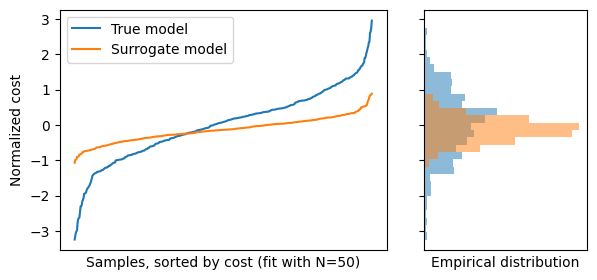
\includegraphics[scale=\distscale]{rand_lin_dist.png}
    \caption*{D-optimal sample selection}
    \vskip\smallskipamount
    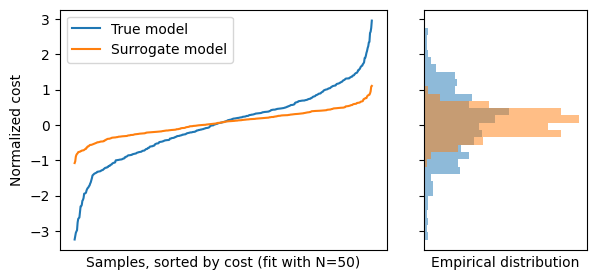
\includegraphics[scale=\distscale]{dopt_dist.png}
    \end{center}
\end{figure}

\begin{figure}[!htbp]
    \begin{center}
    \caption{\label{fig:dist_act} Distributions generated by active learning}
    \caption*{\small Gaussian process baseline}
    \vskip -3\smallskipamount
    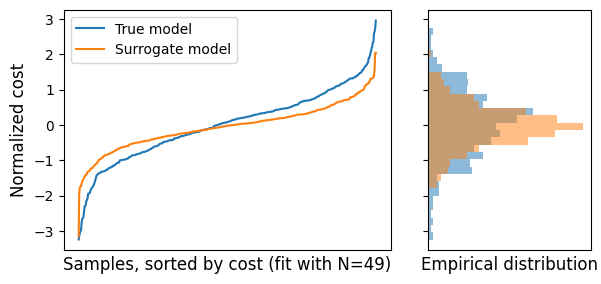
\includegraphics[scale=\distscale]{rand_dist.png}
    \vskip\smallskipamount
    \caption*{Taylor approximation}
    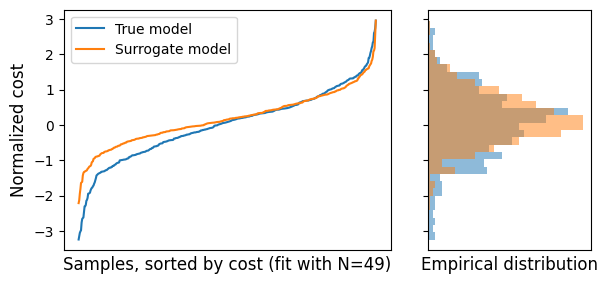
\includegraphics[scale=\distscale]{taylor_dist.png}
    \vskip\smallskipamount
    \caption*{Particle method approximation}
    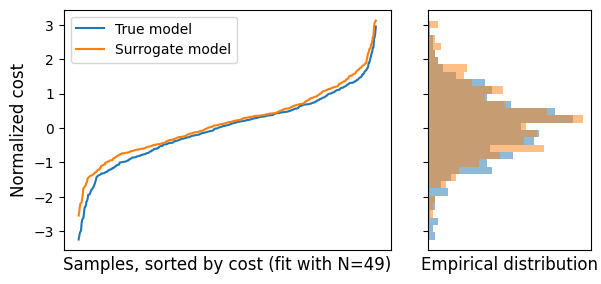
\includegraphics[scale=\distscale]{particle_dist.png}
    \end{center}
\end{figure}

\begin{figure}[!htbp]
    \begin{center}
    \caption{\label{fig:boot_oneshot} Absolute differences in statistics from distributions generated by one-shot selection}
    \caption*{\small One-shot baseline}
    \vskip -3\smallskipamount
    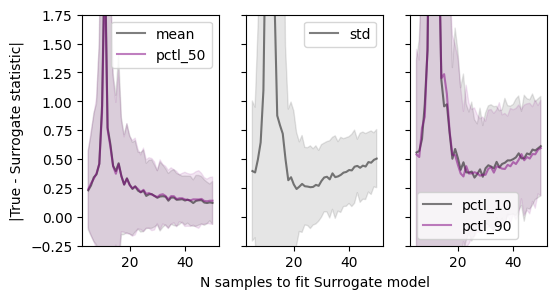
\includegraphics[scale=\bootscale]{rand_lin_statsboot.png}
    \caption*{D-optimal sample selection}
    \vskip\smallskipamount
    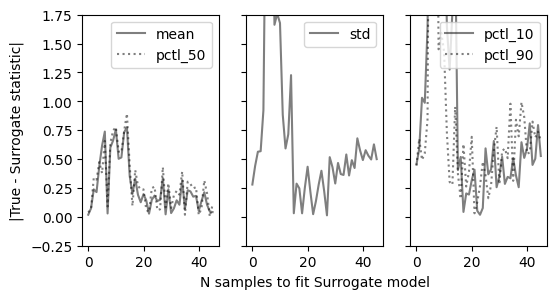
\includegraphics[scale=\bootscale]{dopt_stats.png}
    \end{center}
\end{figure}

\begin{figure}[!htbp]
    \begin{center}
    \caption{\label{fig:boot_act} Absolute differences in statistics from distributions generated by active learning}
    \caption*{\small Gaussian process baseline}
    \vskip -3\smallskipamount
    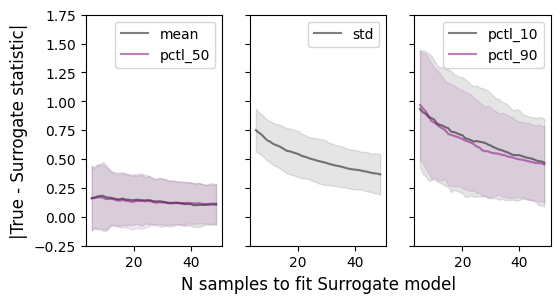
\includegraphics[scale=\bootscale]{rand_statsboot.png}
    \vskip\smallskipamount
    \caption*{Taylor approximation}
    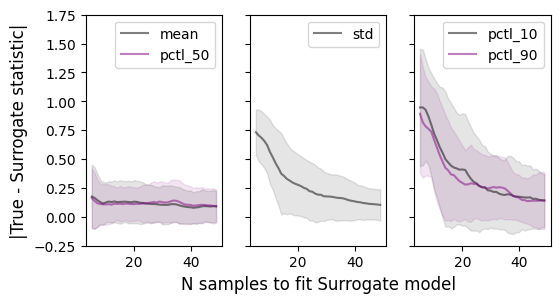
\includegraphics[scale=\bootscale]{taylor_statsboot.png}
    \vskip\smallskipamount
    \caption*{Particle method approximation}
    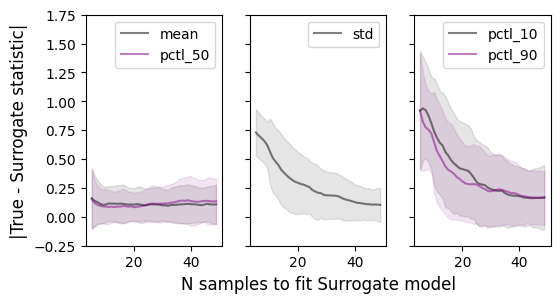
\includegraphics[scale=\bootscale]{particle_statsboot.png}
    \end{center}
\end{figure}


%------------------------------------------------------------------------
\section{Discussion and future work}
\label{sec:conclusion}

Our results demonstrate that complex production cost simulation models can be approximated with simple linear or gaussian process models as a function of encoded stochastic weather and load inputs. It remains to be investigated whether cost model outputs can also be modeled as a function of other PCS inputs like fuel costs.

We suspect that the performance we observe is the result of underlying data and model structures. First, the production cost simulation uses a DC Power Flow model, which requires a linear objective and also linearizes the AC power flow constraints. Hence, it is reasonable to expect that some linear regression model may adequately capture the model behavior. Second, the stochastic profile method models a random walk with a mean reverting term. The process generates each forward step by taking the sum of the previous step, a mean-reverting term, and a random error. It is reasonable to expect that such a structure could be exploited by Gaussian process surrogate models. We propose studying the underlying mechanics leading to our project's outcome in future work.

Another curiosity for future work is to explore the characteristics of these optimal input data samples. We would like to explore the nature of these samples and what they reveal about the core drivers of costs in the cost model. This line of research may reveal key nodes in the network or types of weather patterns that the cost model is particularly sensitive to.

\textcolor{red}{PLACEHOLDER:} Discuss how these methods might be used in a setting where we consider a broader set of expansion scenarios (beyond a single line).

Our PCA encoding strategy captures approximately 2.5\% of the total input data variance. We would like to explore how our results change when we are able to capture a higher share of total variance through an encoding. Such encoding strategies could include wavelet transforms and variational autoencoders for time series data as presented in Desai et. al \cite{desai2021timevae}.

There are several ways we could test the robustness of our results. First, we propose examining our methods under purely random input data, instead of with well-behaved stochastic mean-reversion profiles. \textcolor{red}{TODO:} why would this be helpful? Second, we propose testing these methods under the cannonical two-bus, three-bus, and Tripoli \textcolor{red}{spelling?} networks. Examining our results under these simplified networks will allow us to study the ways in which Gaussian Processes may simulate production cost models. 

Lastly, we propose several extensions to improve and fine tune our sample selection procedures:
\begin{enumerate}
        \item One-shot selection to optimize for quantile regression parameters instead of linear regression parameters as described in Wang et al. (2020) \cite{wang2020optimal}. This strategy could offer a sampling technique to target specific quantiles of the distribution.
        \item Strategies for robust hyperparameter tuning within our Gaussian process kernel as described in Rasmussen et al \cite{Rasmussen}.
        \item Modeling a mixture of Gaussian processes instead of a single Gaussian process as outlined in Blei et al \cite{Blei_2017}.
\end{enumerate}


%------------------------------------------------------------------------
\section{Contributions and acknowledgements}
\label{sec:contrib}
This work is conducted by Erich Trieschman as part of a larger project in collaboration with Kamran Tehranchi. Kamran is responsible for running the production cost model, generating stochastic profile data, and data encoding. All code and results are available on GitHub at \url{https://github.com/etrieschman/grid-planner}.

%%%%%%%%% REFERENCES
{\small
\bibliographystyle{ieee}
\bibliography{egbib}
}

\end{document}
